\documentclass[runningheads]{llncs}
\pdfoutput=1
\usepackage[utf8]{inputenc}
\usepackage{amsmath}
\usepackage{amssymb}
\usepackage{mathpartir}
\usepackage{hyperref}
\usepackage{listings}
\usepackage{graphicx}
\usepackage{comment}
\usepackage{todonotes}
\newcommand\pt{\todo[author=PT,inline]}
\lstdefinelanguage{michelson}{
  basicstyle=\fontsize{8}{9.6}\selectfont,
  morekeywords={parameter,storage,or,unit,mutez,pair,bool,address}, sensitive=false,
  morecomment=[l]{\#},
  morecomment=[\STACK]{/*}{*/},
  morestring=[b]",
}
\lstset{
  language=Caml,
  captionpos=b,
  aboveskip=-\smallskipamount,
  belowskip=-\smallskipamount,
  belowcaptionskip=0pt,
  basicstyle=\fontsize{8}{9.6}\selectfont,
  morekeywords={val}
}

%% structure
\newcommand{\Angle}[1]{\langle#1\rangle}

%% values
\newcommand{\NEG}{\neg}
\newcommand{\CNF}{\wedge}
\newcommand{\DNF}{\vee}
\newcommand{\TRUE}{\text{True}}
\newcommand{\FALSE}{\text{False}}
\newcommand{\EMPTYSTRING}{\text{$""$}}
\newcommand{\STACKCONCAT}{\text{$::$}}
\newcommand{\ZERO}{\text{0}}
\newcommand{\ONE}{\text{1}}
\newcommand{\VAMOUNT}{\text{amount}}
\newcommand{\VCONTRACT}{\text{contract}}

%% contract constants
\newcommand{\CAMOUNT}{\text{amount}}
\newcommand{\CBALANCE}{\text{balance}}
\newcommand{\CSENDER}{\text{sender}}
\newcommand{\CSOURCE}{\text{source}}
\newcommand{\CNOW}{\text{now}}
\newcommand{\CLEVEL}{\text{level}}
\newcommand{\CCHAINID}{\text{chain-id}}
\newcommand{\CSELF}{\text{self}}
\newcommand{\CSELFADDRESS}{\text{self-address}}
\newcommand{\CTOTALVOTINGPOWER}{\text{total-voting-power}}
\newcommand{\CVOTINGPOWER}{\text{voting-power}}

%% contract instructions
\newcommand{\AMOUNT}{\text{AMOUNT}}
\newcommand{\BALANCE}{\text{BALANCE}}
\newcommand{\SENDER}{\text{SENDER}}
\newcommand{\SOURCE}{\text{SOURCE}}
\newcommand{\NOW}{\text{NOW}}
\newcommand{\LEVEL}{\text{LEVEL}}
\newcommand{\CHAINID}{\text{CHAIN-ID}}
\newcommand{\SELF}{\text{SELF}}
\newcommand{\SELFADDRESS}{\text{SELF-ADDRESS}}
\newcommand{\TOTALVOTINGPOWER}{\text{TOTAL-VOTING-POWER}}
\newcommand{\VOTINGPOWER}{\text{VOTING-POWER}}
\newcommand{\MinusBalanceAmount}{\text{BALANCE-AMOUNT}}
%% auction contract
\newcommand{\AuctionOwner}{\text{auction-owner}}
\newcommand{\AuctionBidder}{\text{auction-bidder}}
\newcommand{\AuctionClose}{\text{auction-close}}
\newcommand{\AuctionOpen}{\text{auction-open}}
\newcommand{\AuctionBid}{\text{auction-bid}}

%% system definition
\newcommand{\VAL}{\textbf{v}}
\newcommand{\VAR}{\textbf{x}}
\newcommand{\VARIABLE}{\text{$Var$}}
\newcommand{\CONSTANT}{\text{$Const$}}
\newcommand{\TERM}{\text{$T$}}
\newcommand{\VariableX}{\text{$x$}}
\newcommand{\VariableV}{\text{$v$}}
\newcommand{\VariableK}{\text{$k$}}
\newcommand{\VariableA}{\text{$a$}}
\newcommand{\VariableB}{\text{$b$}}
\newcommand{\ELT}{\text{$Elt$}}
\newcommand{\A}{\text{$A$}}
\newcommand{\B}{\text{$B$}}
\newcommand{\N}{\text{$n$}}
\newcommand{\K}{\text{$k$}}
\newcommand{\V}{\text{$v$}}
\newcommand{\M}{\text{$m$}}
\newcommand{\VariableOne}{\text{$x_1$}}
\newcommand{\VariableTwo}{\text{$x_2$}}
\newcommand{\VariableN}{\text{$x_n$}}
\newcommand{\Constant}{\text{$c$}}
\newcommand{\ConstantOne}{\text{$c_1$}}
\newcommand{\ConstantTwo}{\text{$c_2$}}
\newcommand{\ConstantN}{\text{$c_n$}}
\newcommand{\LIST}{\text{$l$}}
\newcommand{\EMPTYLIST}{\text{$\{\}$}}
\newcommand{\TLIST}{\text{$l'$}}
\newcommand{\HEAD}{\text{$hd$}}
\newcommand{\TAIL}{\text{$tl$}}
\newcommand{\STAIL}{\text{$< tl >$}}
\newcommand{\Term}{\text{$t$}}
\newcommand{\TermOne}{\text{$t_1$}}
\newcommand{\TermTwo}{\text{$t_2$}}
\newcommand{\TermN}{\text{$t_n$}}
\newcommand{\TermB}{\text{$t_b$}}
\newcommand{\STACK}{\text{$S$}}
\newcommand{\EMPTYSTACK}{\text{[ ]}}
\newcommand{\STACKONE}{\text{$S$}}
\newcommand{\STACKTWO}{\text{$S$}}
\newcommand{\STACKN}{\text{$S$}}
\newcommand{\Stack}{\text{$s$}}
\newcommand{\StackOne}{\text{$s_1$}}
\newcommand{\StackTwo}{\text{$s_2$}}
\newcommand{\StackN}{\text{$s_n$}}
\newcommand{\TSTACK}{\text{$S'$}}
\newcommand{\TStack}{\text{$s'$}}
\newcommand{\STATE}{\text{$ST$}}
\newcommand{\STATEONE}{\text{$ST_1$}}
\newcommand{\STATETWO}{\text{$ST_2$}}
\newcommand{\STATEN}{\text{$ST_n$}}
\newcommand{\SYSTEM}{\text{$SE$}}
\newcommand{\INSTRUCTION}{\text{$I$}}
\newcommand{\TINSTRUCTION}{\text{$I'$}}
\newcommand{\INSTRUCTIONONE}{\text{$I1$}}
\newcommand{\INSTRUCTIONTWO}{\text{$I2$}}
\newcommand{\Instruction}{\text{$i$}}
\newcommand{\TInstruction}{\text{$i'$}}
\newcommand{\InstructionOne}{\text{$i_1$}}
\newcommand{\InstructionTwo}{\text{$i_2$}}
\newcommand{\InstructionN}{\text{$i_n$}}
\newcommand{\Invariant}{\text{$Iv$}}
\newcommand{\PREDICATE}{\text{$P$}}
\newcommand{\PREDICATEA}{\text{$P_A$}}
\newcommand{\PREDICATEB}{\text{$P_B$}}
\newcommand{\Predicate}{\text{$p$}}
\newcommand{\Failwith}{\text{$Failwith$}}
\newcommand{\PredicateOne}{\text{$p_1$}}
\newcommand{\PredicateTwo}{\text{$p_2$}}
\newcommand{\PredicateN}{\text{$p_n$}}
\newcommand{\SETA}{\text{$\mathcal{A}$}}
\newcommand{\SETAAUCTION}{\text{$\mathcal{A}_{auction}$}}
\newcommand{\SETPOST}{\text{$\mathcal{A'}$}}
\newcommand{\SETPOSTAUCTION}{\text{$\mathcal{A'}_{auction}$}}
\newcommand{\EMPTY}{\text{$\O$}}
\newcommand{\PCreate}{\text{$P_{Create}$}}
\newcommand{\PBidding}{\text{$P_{Bidding}$}}
\newcommand{\PClose}{\text{$P_{Close}$}}
\newcommand{\SE}{\text{SE}}
\newcommand{\SINIT}{\text{$s_{init}$}}
\newcommand{\SFINAL}{\text{$s_{final}$}}
\newcommand{\FMAP}{\textbf{map}}
\newcommand{\MAPA}{\textbf{$map_A$}}
\newcommand{\MAPB}{\textbf{$map_B$}}
\newcommand{\MapBidding}{\textbf{$map_{bidding}$}}
\newcommand{\MapCreate}{\textbf{$map_{create}$}}
\newcommand{\MapClose}{\textbf{$map_{close}$}}
\newcommand{\MAPER}{\text{$\overline{\textbf{map}}$}}


%% operation
\newcommand{\CONS}{\text{cons}}
\newcommand{\NIL}{\text{nil}}
\newcommand{\PLUS}{\textbf{+}}
\newcommand{\MINUS}{\textbf{-}}
\newcommand{\EQUAL}{\textbf{=}}
\newcommand{\LESS}{\textbf{$<$}}
\newcommand{\LESSEQUAL}{\textbf{$<=$}}
\newcommand{\MORE}{\textbf{$>$}}
\newcommand{\MOREEQUAL}{\textbf{$>=$}}

%% instructions
\newcommand{\UNIT}{\text{Unit}}
\newcommand{\PAIR}{\text{Pair}}
\newcommand{\LEFT}{\text{Left}}
\newcommand{\RIGHT}{\text{Right}}
\newcommand{\SOME}{\text{Some}}
\newcommand{\NONE}{\text{None}}
\newcommand{\ADD}{\text{ADD}}
\newcommand{\DROP}{\text{DROP}}
\newcommand{\LOOP}{\text{LOOP}}
\newcommand{\FAILWITH}{\text{FAILWITH}}
\newcommand{\TRANSFER}[2]{\text{Transfer($#1$, $#2$)}}
\newcommand{\CONTRACT}{\text{CONTRACT}}
\newcommand{\CAR}{\text{CAR}}
\newcommand{\EXEC}{\text{EXEC}}
\newcommand{\APPLY}{\text{APPLY}}
\newcommand{\IF}{\text{IF}}
\newcommand{\IFLEFT}{\text{IF-LEFT}}
\newcommand{\IFRIGHT}{\text{IF-RIGHT}}
\newcommand{\IFCONS}{\text{IF-CONS}}
\newcommand{\ITER}{\text{ITER}}
\newcommand{\TITER}{\text{ITER'}}
\newcommand{\DIG}{\text{DIG}}
\newcommand{\DIP}{\text{DIP}}
\newcommand{\DIPN}{\text{DIP n}}
\newcommand{\TDIP}{\text{DIP'}}
\newcommand{\ABS}{\text{ABS}}
\newcommand{\COMPARE}{\text{COMPARE}}
\newcommand{\TCOMPARE}{\text{COMPARE'}}
\newcommand{\HASHKEY}{\text{HASH-KEY}}
\newcommand{\CONCAT}{\text{CONCAT}}
\newcommand{\TCONCAT}{\text{CONCAT'}}
\newcommand{\MEN}{\text{MEN}}
\newcommand{\TMEN}{\text{MEN'}}
\newcommand{\TMAP}{\text{MAP'}}
\newcommand{\PUSH}{\text{PUSH}}
\newcommand{\XOR}{\text{XOR}}
\newcommand{\MAP}{\textbf{MAP}}
\newcommand{\LAMBDA}{\text{LAMBDA}}


%symbols
\newcommand{\Overline}[1]{\text{$\overline{#1}$}}
\newcommand{\Mapsto}{\text{$\mapsto$}}
\newcommand{\Mid}{\text{$\mid$}}
\newcommand{\Mathcal}[1]{\text{$\mathcal{#1}$}}
\newcommand{\Models}{\text{$\models$}}
\newcommand{\SRightarrow}{\text{$\rightarrow$}}
\newcommand{\NSRightarrow}{\text{$\nrightarrow$}}
\newcommand{\Wedge}{\text{$\wedge$}}
\newcommand{\At}{\text{$@$}}
\newcommand{\Subseteq}{\text{$\subseteq$}}
\newcommand{\Vee}{\text{$\vee$}}
%\newcommand{\Cup}{\text{$\cup$}}
\newcommand{\STRINGCONCAT}{\text{$\hat{}$}}
\newcommand{\DOT}{\text{$...$}}


%% functions
\newcommand{\FABS}[1]{\text{abs($#1$)}}
\newcommand{\FXOR}{\text{xor}}
\newcommand{\FHASHKEY}[1]{\text{hash-key($#1$)}}
\newcommand{\FCONCAT}[1]{\text{concat($#1$)}}
\newcommand{\FGetTy}[1]{\text{get-ty($#1$)}}
\newcommand{\FLEN}[1]{\text{len($#1$)}}
\newcommand{\FAND}{\text{and}}
\newcommand{\FOR}{\text{or}}
\newcommand{\FNOT}{\text{not}}
\newcommand{\GETCONTRACTTYPE}{\text{get-contract-type}}
\newcommand{\UNOP}{\text{unop}}
\newcommand{\BINOP}{\text{binop}}



%% transition relations
\newcommand{\StateTrans}{\text{$\longrightarrow_S$}}
\newcommand{\ExprTrans}{\text{$\longrightarrow_E$}}
\newcommand{\SystemTrans}{\text{$\longrightarrow$}}


%% types
\newcommand\TEnv{\Gamma}
\newcommand\JTypeCode[2]{\vdash_C#1 : #2}
\newcommand\JTypeValue[2]{\vdash_V#1 : #2}
\newcommand\JTypeExpr[3]{#1 \vdash #2 : #3}
\newcommand{\TY}{\text{ty}}
\newcommand{\TYF}{\text{ty$_{1}$}}
\newcommand{\TYS}{\text{ty$_{2}$}}
\newcommand{\TYT}{\text{ty$_{3}$}}
\newcommand{\TYA}{\text{A}}
\newcommand{\TYB}{\text{B}}
\newcommand{\TYC}{\text{C}}
%% standard types
\newcommand{\TBOOL}{\text{bool}}
\newcommand{\TOR}{\text{or}}
\newcommand{\TYLIST}{\text{list}}
\newcommand{\TUNIT}{\text{unit}}
\newcommand{\TPAIR}{\text{pair}}
\newcommand{\TOPTION}{\text{option}}
\newcommand{\TMUTEZ}{\text{mutez}}
\newcommand{\TSTR}{\text{string}}
\newcommand{\TINT}{\text{int}}
\newcommand{\TNAT}{\text{nat}}
\newcommand{\TKEY}{\text{key}}
\newcommand{\TKEYHASH}{\text{key-hash}}
\newcommand{\TSIG}{\text{signature}}
\newcommand{\TADDR}{\text{address}}
\newcommand{\TTIME}{\text{timestamp}}
\newcommand{\TCONTRACT}{\text{contract}}
\newcommand{\TCHAINID}{\text{chain-id}}
\newcommand{\TLAMBDA}{\text{lambda}}







%% typing related
\newcommand{\EmptyEnv}{\cdot}

%% evaluation contexts
\newcommand\EC[1]{\epsilon[#1]}

%% metavariables


%%% Local Variables:
%%% mode: latex
%%% TeX-master: "paper"
%%% End:



\begin{document}
%
\title{Symblic Execution Model}
%
%\titlerunning{Abbreviated paper title}
% If the paper title is too long for the running head, you can set
% an abbreviated paper title here
%
\author{Thi Thu Ha Doan\orcidID{0000-0001-7524-4497}\and
  Peter Thiemann\orcidID{0000-0002-9000-1239}}

%
\authorrunning{Ha Doan, P. Thiemann}
% First names are abbreviated in the running head.
% If there are more than two authors, 'et al.' is used.
%
\institute{University of Freiburg, Germany \\
  \email{\{doanha,thiemann\}@informatik.uni-freiburg.de}
}
%
\maketitle              % typeset the header of the contribution
%
\begin{abstract}
 

\keywords{}
\end{abstract}

%
%
%
\section{Introduction}
\label{sec:introduction}

\section{Symblic Execution Model}
\label{sec:symblic-execution-model}

Let $\STACK = \TermOne \STACKCONCAT \TermTwo \STACKCONCAT \DOT
\STACKCONCAT \EMPTYSTACK$ be a stack, where elements are terms.
\pt{elements are types paired with terms}
\\
Let $\INSTRUCTION = \InstructionOne; \InstructionTwo; \DOT; \InstructionN$ be a sequence of instructions. 
\\
Let \PREDICATE\ be a predicate. 

\begin{definition}
A system state of the symbolic execution is a tuple $\STATE =
[\INSTRUCTION, \STACK, \TSTACK, \PREDICATE]$, where \STACK\ is the
main stack and \TSTACK\ is a temporary stack. 
\end{definition}

Let $\SYSTEM = \{\STATEONE, \STATETWO, \DOT, \STATEN \}$ range over sets of system states.
\\
\\
Let $S_{init}$  be the initial state.\pt{you say
  ``state'', but what you give is a stack}
\begin{itemize}
\item[]  $S_{init}$ = (Pair $Par$ \Term) \STACKCONCAT\ \EMPTYSTACK
\end{itemize}
 \todo[author=PT,inline]{what is Par, ops,  and  what is $t$?}



\noindent Let $S_{final}$  be the final state. 

\begin{itemize}
\item[]  $S_{final}$ = (\PAIR\ $ops$ $t'$) \STACKCONCAT\ \EMPTYSTACK
\end{itemize}

%Where $t$ and $t'$ represent the storage and have the same structure.

%Postcondition

%(t.x = t'.x)


\begin{figure} []
\begin{align*}
T, U &::= \\
   &\Mid\ \langle \text{comparable type}\rangle \\
   &\Mid\ \text{option} \langle\text{type}\rangle \\
   &\Mid\ \text{list} \langle\text{type}\rangle \\
   &\Mid\ \text{set} \langle\text{comparable type}\rangle \\
   &\Mid\ \text{operation} \\
   &\Mid\ \text{contract} \langle\text{type}\rangle \\
   &\Mid\ \text{ticket} \langle\text{comparable type}\rangle \\
   &\Mid\ \text{pair} \langle\text{type}\rangle \langle\text{type}\rangle \\
   &\Mid\ \text{or} \langle\text{type}\rangle \langle\text{type}\rangle \\
   &\Mid\ \text{lambda} \langle\text{type}\rangle \langle\text{type}\rangle \\
   &\Mid\ \text{map} \langle\text{comparable type}\rangle \langle\text{type}\rangle \\
   &\Mid\ \text{big-map} \langle\text{comparable type}\rangle \langle\text{type}\rangle \\
   &\Mid\ \text{bls12-381-g1} \\
   &\Mid\ \text{bls12-381-g2} \\
   &\Mid\ \text{bls12-381-fr} \\
   &\Mid\ \text{sapling-transaction} \langle\text{natural number constant}\rangle \\
   &\Mid\ \text{sapling-state} \langle\text{natural number constant}\rangle \\
   &\Mid\ \text{chest} \\
   &\Mid\ \text{chest-key} \\
\langle\text{comparable type}\rangle ::= \\
   &\Mid\ \text{unit} \\
   &\Mid\ \text{never} \\
   &\Mid\ \text{bool} \\
   &\Mid\ \text{int}\\
   &\Mid\ \text{nat}\\
   &\Mid\ \text{string}\\
   &\Mid\ \text{chain-id}\\
   &\Mid\ \text{bytes}\\
   &\Mid\ \text{mutez}\\
   &\Mid\ \text{key-hash}\\
   &\Mid\ \text{key}\\
   &\Mid\ \text{signature}\\
   &\Mid\ \text{timestamp}\\
   &\Mid\ \text{address}\\
   &\Mid\ \text{tx-rollup-l2-address}\\
   &\Mid\ \text{option} \langle\text{comparable type}\rangle\\
   &\Mid\ \text{or} \langle\text{comparable type}\rangle \langle\text{comparable type}\rangle\\
   &\Mid\ \text{pair} \langle\text{comparable type}\rangle \langle\text{comparable type}\rangle \DOT \\
\end{align*}
\caption{Types}
\label{fig:type}
\end{figure}

\begin{figure}[h]
\begin{align*}
\text{t} &::= \\
   &\Mid\ \langle \text{variable} \rangle \\
   &\Mid\ \langle \text{account constant} \rangle \\
   &\Mid\ \langle \text{int constant} \rangle \\
   &\Mid\ \langle \text{string constant} \rangle \\
   &\Mid\ \langle \text{byte sequence constant} \rangle \\
   &\Mid\ \UNIT \\
   &\Mid\ \TRUE \\
   &\Mid\ \FALSE \\
   &\Mid\ \PAIR\ \text{t1 t2}\\
   &\Mid\ \LEFT\ \text{t}\\
   &\Mid\ \RIGHT\ \text{t}\\ 
   &\Mid\ \SOME\ \text{t}\\
   &\Mid\ \NONE \\
   &\Mid\ \text{\{t ; ... \}}\\
   &\Mid\ \text{\{ Elt t1 t2 ; ... \}}\\
   &\Mid\ \{ \langle\text{instruction}\rangle; ... \}   \\
\langle \text{variable} \rangle &::= \\ 
   &\Mid\ \VAR\\
\langle \text{account constant} \rangle &::= \\ 
   &\Mid\ \text{balance} \\
   &\Mid\ \text{amount} \\
   &\Mid\ \text{sender} \\
   &\Mid\ \text{source} \\
   &\Mid\ \text{now} \\
   &\Mid\ \text{level} \\
   &\Mid\ \text{chain-id} \\
   &\Mid\ \text{self}  \\
   &\Mid\ \text{self-address}  \\
   &\Mid\ \text{total-voting-power}  \\
   &\Mid\ \text{voting-power}  \\
\langle \text{natural number constant} \rangle &::= \\ 
   &\Mid\ \text {[0-9]+} \\
\langle \text{int constant} \rangle &::= \\
  &\Mid\ \langle \text{natural number constant} \rangle \\
  &\Mid\ \text{-} \langle \text{natural number constant} \rangle \\
\langle\text{string constant}\rangle &::= \\
  &\Mid\ \text{"} \langle \text{string content}\rangle\text{*"} \\
\langle\text{instruction}\rangle &::= \\
  &\Mid\ \DROP \\
  &\Mid\ \DROP \langle\text{natural number constant}\rangle \\
  &\text{...}
\end{align*}
\caption{Terms}
\label{fig:term}
\end{figure}


\begin{figure}[h]
\begin{align*}
\text{p} &::= \\
   &\Mid\ \langle \text{atomic formula} \rangle \\
   &\Mid\ \NEG\ \text{p} \
   \Mid\ \text{p}\ \CNF\ \text{q} \
   \Mid\ \text{p}\ \DNF\ \text{q} \\
\langle \text{atomic formula} \rangle &::= \\ 
    &\Mid\ \langle \text{butop} \rangle \langle \text{bterm} \rangle\\ 
   &\Mid\  \langle \text{bterm} \rangle  \langle \text{biop} \rangle \langle \text{bterm} \rangle\\ 
\langle \text{butop} \rangle &::= \\
   &\Mid\ \text{not} \\
\langle \text{biop} \rangle &::= \\
   &\Mid\ \text{$=$} \
   \Mid\ \text{$>$} \
   \Mid\ \text{$<$} \
   \Mid\ \text{$>=$} \
   \Mid\ \text{$=<$} \
   \Mid\ \text{$!=$} \\
   &\Mid\ \text{and}\ \Mid\ \text{or}\ \Mid\ \text{xor}\\
\langle \text{bterm} \rangle &::= \\ 
   &\Mid\ \text{t} \\
   &\Mid\ \langle \text{unop} \rangle \text{t} \\ 
   &\Mid\ \text{t}\ \langle \text{binop} \rangle \text{t}\\  
\langle \text{unop} \rangle &::= \\ 
   &\Mid\ \text{abs} \\
   &\Mid\ \text{size} \\
   &\Mid\ \text{int} \\
   &\Mid\ \text{contract}  \langle \text{type} \rangle \\
   &\Mid\ \text{isleft} \\
   &\Mid\ \text{isnone} \\
   &\Mid\ \text{neg} \\
   &\Mid\ \text{blake2b} \\
   &\Mid\ \text{hash-key} \\
   &\Mid\ \text{keccak} \\
   &\Mid\ \text{pairing-check} \\
   &\Mid\ \text{sha256} \\
   &\Mid\ \text{sha3} \\
   &\Mid\ \text{sha512} \\
   &\Mid\ \text{implicit-account} \\
   &\Mid\ \text{check-sig} \\
\langle \text{bitop} \rangle &::= \\ 
   &\Mid\ \text{+}\ \Mid\ \text{-}\ \Mid\ \text{*}\ \Mid\ \text{/}
\end{align*}
\caption{Predicates}
\label{fig:predicate}
\end{figure}


\paragraph{Sequence actions.}
\begin{figure}[h]
\center
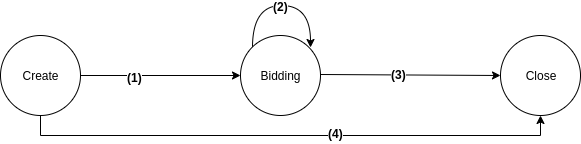
\includegraphics[width= 10 cm]{life-cycle-1}
\caption{Life-cycle for the auction contract.}
\label{fca1}
\end{figure} 

\pagebreak
\section{Rules}
The set of instructions is divided into two groups \INSTRUCTION\ and \TINSTRUCTION. Given an instruction \Instruction, \TInstruction\ is a copy version of \Instruction, where \Instruction\ operates on the main stack \STACK\ and \TInstruction\ operates only on the temporary stack \TSTACK.

The rule semantic is defined by several kinds of transitions:
\begin{enumerate}
\item \ExprTrans\ single-step evaluation of an expression in a system state,
\item \StateTrans\ internal transitions of a system state,
  \pt{this relation should be non-deterministic as shown for
    instructions \IF, \IFLEFT, and \LOOP; this approach enables us to
    simplify the rule for \DIP}
\item \SystemTrans\ symbolic system transitions.
\end{enumerate}

\subsubsection{System rules}
\begin{mathpar}
\inferrule[INVALID-PRE]
  { \NEG\ \PREDICATE
  }{
  \{[\INSTRUCTION, \STACK, \TSTACK, \PREDICATE]\} \cup \SYSTEM \SystemTrans \SYSTEM}
\end{mathpar}

\subsubsection{Instruction rules}
\paragraph{Control structures}
%EXE
\begin{mathpar}
  \inferrule[EXEC]
  {
    [\INSTRUCTIONONE, \StackOne \STACKCONCAT \EMPTYSTACK, \EMPTYSTACK,
    Q]
    \StateTrans^*
    [ \EMPTYSTACK, \StackOne' \STACKCONCAT \EMPTYSTACK, \EMPTYSTACK, Q']
  }{
    [(\EXEC; \INSTRUCTION),   \{\INSTRUCTIONONE\} \STACKCONCAT
    \StackOne \STACKCONCAT \STACK, \TSTACK, \PREDICATE \wedge Q] 
    \StateTrans
    [ \INSTRUCTION, \StackOne' \STACKCONCAT \STACK, \TSTACK,
    \PREDICATE \wedge Q']}
\end{mathpar}

%APPLY
\begin{mathpar}
  \inferrule[APPLY]
  {
  }{
    \text{[(\APPLY; \INSTRUCTION), \StackOne\ \STACKCONCAT\ \{\INSTRUCTIONONE\} \STACKCONCAT\ \STACK, \TSTACK, \PREDICATE]} \StateTrans\ \text{[\INSTRUCTION, \{\PUSH\ (\FGetTy\StackOne)\ \StackOne; \IPAIR; \INSTRUCTIONONE\} \STACKCONCAT\ \STACK, \TSTACK, \PREDICATE]}}
\end{mathpar}

%LAMBLA
\begin{mathpar}
  \inferrule[LAMBDA]
  {  
  }{
    [(\LAMBDA\ \TYF\ \TYS\ \{ \INSTRUCTIONONE \} ; \INSTRUCTION),\STACK, \TSTACK, \PREDICATE] \StateTrans\ [\INSTRUCTION, \{ \INSTRUCTIONONE \}\ \STACKCONCAT\ \STACK, \TSTACK, \PREDICATE]}
\end{mathpar}

%IF
\begin{mathpar}
  \inferrule[IF-TRUE]
  {  
  }{
    [(\IF\ \INSTRUCTIONONE\  \INSTRUCTIONTWO; \INSTRUCTION),
    \StackOne\ \STACKCONCAT\ \STACK, \TSTACK, \PREDICATE]
    \SystemTrans
    [\INSTRUCTIONONE, \STACK, \TSTACK, \PREDICATE\ \Wedge\ \StackOne]
  }

  \inferrule[IF-FALSE]
  {  
  }{
    [(\IF\ \INSTRUCTIONONE\  \INSTRUCTIONTWO; \INSTRUCTION),
    \StackOne\ \STACKCONCAT\ \STACK, \TSTACK, \PREDICATE]
    \SystemTrans
   [\INSTRUCTIONTWO, \STACK, \TSTACK, \PREDICATE\ \Wedge\ \NEG\
   \StackOne]
 }
\end{mathpar}


%IF-LEFT-LEFT
\begin{mathpar}
  \inferrule[IF-LEFT-LEFT]
  {  
  }{
    [(\IFLEFT\ \INSTRUCTIONONE\ \INSTRUCTIONTWO; \INSTRUCTION),
    \StackOne \STACKCONCAT \STACK, \TSTACK, \PREDICATE]
    \StateTrans
    [\INSTRUCTIONONE, \VariableX\ \STACKCONCAT\ \STACK, \TSTACK,
    \PREDICATE \wedge (\StackOne\ \EQUAL\ \LEFT\ \VariableX)]
  }
\end{mathpar}

%IF-LEFT-RIGHT
\begin{mathpar}
  \inferrule[IF-LEFT-RIGHT]
  {  
  }{
    [(\IFLEFT\ \INSTRUCTIONONE\  \INSTRUCTIONTWO; \INSTRUCTION),
    \StackOne \STACKCONCAT \STACK, \TSTACK, \PREDICATE]
    \StateTrans
    [\INSTRUCTIONTWO, \VariableX\ \STACKCONCAT\ \STACK, \TSTACK, \PREDICATE \wedge (\StackOne\ \EQUAL\ \RIGHT\ \VariableX)]
  }
\end{mathpar}



%IF-CONS-EMPTY
\begin{mathpar}
  \inferrule[IF-CONS-EMPTY]
  {  
  }{
    [(\IFCONS\ \INSTRUCTIONONE\  \INSTRUCTIONTWO\ ; \INSTRUCTION),  \EMPTYLIST\ \STACKCONCAT\ \STACK, \TSTACK, \PREDICATE] \StateTrans\  [\INSTRUCTIONTWO\ ; \INSTRUCTION, \STACK, \TSTACK, \PREDICATE]}
\end{mathpar}

%IF-LEFT-NONEMPTY
\begin{mathpar}
  \inferrule[IF-CONS-NONEMPTY]
  {  
  }{
    [(\IFCONS\ \INSTRUCTIONONE\  \INSTRUCTIONTWO\ ; \INSTRUCTION),  \{\HEAD\ ; \STAIL \}\ \STACKCONCAT\ \STACK, \TSTACK, \PREDICATE]\ \StateTrans\  [\INSTRUCTIONONE\ ; \INSTRUCTION, \HEAD\ \STACKCONCAT\ \TAIL\ \STACKCONCAT\ \STACK, \TSTACK, \PREDICATE]}
\end{mathpar}


%IF_CONS
\begin{mathpar}
  \inferrule[IF-CONS]
  {  
  }{
    \{[(\IFCONS\ \INSTRUCTIONONE\  \INSTRUCTIONTWO\ ; \INSTRUCTION),  \StackOne\ \STACKCONCAT\ \STACK, \TSTACK, \PREDICATE], \SYSTEM\}\ \SystemTrans\  \\ \{[\INSTRUCTIONTWO\ ; \INSTRUCTION, \STACK, \TSTACK, \PREDICATE\ \Wedge\ (\StackOne\ \EQUAL\ \EMPTYLIST)], [\INSTRUCTIONONE, \HEAD\ \STACKCONCAT\ \TAIL\ \STACKCONCAT\ \STACK, \TSTACK, \PREDICATE\ \Wedge\ ( \StackOne\ \EQUAL\ \{\HEAD\ ; \STAIL \})], \SYSTEM\}}
\end{mathpar}

%IF_NON
\begin{mathpar}
  \inferrule[IF-NONE]
  {  
  }{
    \{[(\IFNONE\ \INSTRUCTIONONE\  \INSTRUCTIONTWO\ ; \INSTRUCTION),  \StackOne\ \STACKCONCAT\ \STACK, \TSTACK, \PREDICATE], \SYSTEM\}\ \SystemTrans\  \\ \{[\INSTRUCTIONONE\ ; \INSTRUCTION, \STACK, \TSTACK, \PREDICATE\ \Wedge\ \StackOne\ \EQUAL\ \NONE], [\INSTRUCTIONTWO,  \VariableX\ \STACKCONCAT\ \STACK, \TSTACK, \PREDICATE\ \Wedge\ ( \StackOne\ \EQUAL\ \SOME\ \VariableX], \SYSTEM\}}
\end{mathpar}


%LOOP
\begin{mathpar}
  \inferrule[LOOP-TRUE]
  {  
  }{
    [(\LOOP\ \INSTRUCTIONONE; \INSTRUCTION),  \StackOne\
    \STACKCONCAT\ \STACK, \TSTACK, \PREDICATE]
    \SystemTrans
    [(\INSTRUCTIONONE; \LOOP\ \INSTRUCTIONONE; \INSTRUCTION),
    \STACK, \TSTACK, \PREDICATE \wedge \StackOne]
  }

  \inferrule[LOOP-FALSE]
  {  
  }{
    [(\LOOP\ \INSTRUCTIONONE; \INSTRUCTION),  \StackOne\ \STACKCONCAT\
    \STACK, \TSTACK, \PREDICATE]
    \SystemTrans
   [\INSTRUCTION, \STACK, \TSTACK, \PREDICATE \wedge
   (\NEG\StackOne)]
   }
\end{mathpar}

% \begin{mathpar}
%   \inferrule[LOOP]
%   {  
%   }{
%     \{[(\LOOP\ \INSTRUCTIONONE; \INSTRUCTION),  \StackOne\ \STACKCONCAT\ \STACK, \TSTACK, \PREDICATE], \SYSTEM\} \SystemTrans \\ \{[(\INSTRUCTIONONE; \LOOP\ \INSTRUCTIONONE; \INSTRUCTION), \STACK, \TSTACK, \PREDICATE\ \Wedge\ \StackOne], [\INSTRUCTION, \STACK, \TSTACK, \PREDICATE\ \Wedge\ (\NEG\StackOne)], \SYSTEM\}}
% \end{mathpar}


\begin{mathpar}
  \inferrule[ITER]
  {  
  }{
    \{[(\ITER\ \INSTRUCTIONONE ; \INSTRUCTION), \StackOne\ \STACKCONCAT\ \STACK, \TSTACK, \PREDICATE], \SYSTEM\} \StateTrans \\ \{[\INSTRUCTION, \STACK,  \TSTACK, \PREDICATE\ \Wedge\  (\StackOne\ \EQUAL\ \EMPTYLIST)], [(\TITER\ \INSTRUCTIONONE ; \INSTRUCTION), \STACK, \StackOne\ \STACKCONCAT\ \TSTACK, \PREDICATE\ \Wedge\ \NEG\ (\StackOne\ \EQUAL\ \EMPTYLIST)], \SYSTEM\}
  }
\end{mathpar}

\begin{mathpar}
  \inferrule[ITER']
  {  
  }{
    \{[(\TITER\ \INSTRUCTIONONE ; \INSTRUCTION), \STACK, \StackOne\ \STACKCONCAT\ \TSTACK, \PREDICATE], \SYSTEM \} \SystemTrans \\ \{[\INSTRUCTION, \STACK,  \TSTACK, \PREDICATE\ \Wedge\  (\StackOne\ \EQUAL\ \EMPTYLIST)], [(\INSTRUCTIONONE; \TITER\ \INSTRUCTIONONE ; \INSTRUCTION), \HEAD\ \STACKCONCAT\ \STACK,  \{\TAIL\} \STACKCONCAT\ \TSTACK, \PREDICATE\ \Wedge\ ( \StackOne\ \EQUAL\ \{\HEAD\ ; \STAIL \})], \SYSTEM\}
  }
\end{mathpar}

\paragraph{Stack Manipulation}
%DIG
\begin{mathpar}
\inferrule[DIG]
  {
   \FLEN\A\ \EQUAL\ \N
  }
  {[(\DIG\ \N ; \INSTRUCTION), \A\ \At\ \StackOne\ \STACKCONCAT\ \B, \TSTACK, \PREDICATE] \StateTrans 
[\INSTRUCTION, \StackOne\ \STACKCONCAT\ \A\ \At\ \B, \TSTACK, \PREDICATE]}
\end{mathpar}

%DIP
\begin{mathpar}
  \inferrule[DIP]
  {
    [\INSTRUCTIONONE,  \STACK, \EMPTYSTACK, Q]
    \StateTrans^*
    [\EMPTYSTACK,  \STACK_1, \EMPTYSTACK, Q']
  }
  {[(\DIP\ \INSTRUCTIONONE; \INSTRUCTION), \StackOne \STACKCONCAT
    \STACK, \TSTACK, \PREDICATE \wedge Q]
    \StateTrans 
    [\INSTRUCTION, \STACK_1,
    \TSTACK, \PREDICATE \wedge Q']
  }
\end{mathpar}

% \begin{mathpar}
% \inferrule[DIP']
%   { 
%   }
%   {\text{[(\TDIP\ \INSTRUCTIONONE; \INSTRUCTION), \STACK, \StackOne\ \STACKCONCAT\ \TSTACK, \PREDICATE]} \StateTrans 
% \text{[\INSTRUCTION, \StackOne\ \STACKCONCAT\ \STACK, \TSTACK, \PREDICATE]}}
% \end{mathpar}

%DIP n
\begin{mathpar}
\inferrule[DIP n]
  { 
     \text{\FLEN\A\ \EQUAL\ \N}
  }
  {\text{[(\DIP\ \N\ \INSTRUCTIONONE; \INSTRUCTION), \A\ \At\ \B, \TSTACK, \PREDICATE]} \StateTrans 
\text{[(\INSTRUCTIONONE; \TDIP\ \N\ \INSTRUCTIONONE; \INSTRUCTION), \B, \A\ \At\ \TSTACK, \PREDICATE]}}
\end{mathpar}


\begin{mathpar}
\inferrule[DIP' n]
  {
   \text{\FLEN\A\ \EQUAL\ \N}
  }
  {\text{[(\TDIP\ \N\ \INSTRUCTIONONE; \INSTRUCTION), \STACK, \A\ \At \TSTACK, \PREDICATE]} \StateTrans 
\text{[\INSTRUCTION, \A\ \At\ \STACK, \TSTACK, \PREDICATE]}}
\end{mathpar}


%PUSH
\begin{mathpar}
  \inferrule[PUSH]
  {  
  }{
    [(\PUSH\ \TYF\ \VariableX\ ; \INSTRUCTION),\STACK, \TSTACK, \PREDICATE] \StateTrans\ [\INSTRUCTION, \VariableX\ \STACKCONCAT\ \STACK, \TSTACK, \PREDICATE]}
\end{mathpar}


\paragraph{Arithmetic operations}
%ADD
\begin{mathpar}
\inferrule[ADD]
  {
  }
  {\text{[(\ADD\ ; \INSTRUCTION), \StackOne\ \STACKCONCAT\ \StackTwo\ \STACKCONCAT\ \STACK, \TSTACK, \PREDICATE]} \StateTrans 
\text{[\INSTRUCTION, \VariableX\ \STACKCONCAT\ \STACK, \TSTACK, \PREDICATE \Wedge\ (\VariableX\ \EQUAL\ \StackOne\ \PLUS\ \StackTwo)]}}
\end{mathpar}

%ABS
\begin{mathpar}
\inferrule[ABS]
  {
  }
  {
    [(\ABS\ ; \INSTRUCTION), \StackOne \STACKCONCAT \STACK, \TSTACK,
    \PREDICATE]
    \StateTrans
    [\INSTRUCTION, \VariableX \STACKCONCAT \STACK, \TSTACK,
    \PREDICATE \wedge (\StackOne \ge 0 \Rightarrow \VariableX =
    \StackOne) \wedge (\StackOne <0 \Rightarrow \VariableX = -\StackOne)]
 }
\end{mathpar}

% COMPARE
\pt{I think \COMPARE\ can be simplified as follows}
\begin{mathpar}
\inferrule[COMPARE]
  {
  }
  {
    [(\COMPARE ; \INSTRUCTION), \StackOne \STACKCONCAT \StackTwo
    \STACKCONCAT \STACK, \TSTACK, \PREDICATE]
    \SystemTrans \\
    [\INSTRUCTION, \VariableX \STACKCONCAT \STACK, \TSTACK, \PREDICATE
    \wedge (\StackOne > \StackTwo \Leftrightarrow \VariableX = 1)
    \wedge (\StackOne = \StackTwo \Leftrightarrow \VariableX = 0)
    \wedge (\StackOne < \StackTwo \Leftrightarrow \VariableX = -1)]
    }
\end{mathpar}


% %COMPARE
% \begin{mathpar}
% \inferrule[COMPARE]
%   {
%   }
%   {[(\COMPARE\ ; \INSTRUCTION), \SOME\ \VariableX\ \STACKCONCAT\ \SOME\ \VariableY\ \STACKCONCAT\ \STACK, \TSTACK, \PREDICATE] \StateTrans \\
% [(\COMPARE\ ; \INSTRUCTION), \VariableX\ \STACKCONCAT\ \VariableY\ \STACKCONCAT\  \STACK, \TSTACK, \PREDICATE \Wedge\ (\StackOne\ \MORE\ \StackTwo)]}
% \end{mathpar}


% \begin{mathpar}
% \inferrule[COMPARE]
%   {
%   }
%   {\{[(\COMPARE\ ; \INSTRUCTION), \StackOne\ \STACKCONCAT\ \StackTwo\ \STACKCONCAT\ \STACK, \TSTACK, \PREDICATE], \SYSTEM\} \SystemTrans \\
% \{[\INSTRUCTION, \ONE\ \STACKCONCAT\ \STACK, \TSTACK, \PREDICATE \Wedge\ (\StackOne\ \MORE\ \StackTwo) \Wedge\ (\FGetTy \StackOne\ \EQUAL\ \TINT) \Wedge\ (\FGetTy \StackTwo\ \EQUAL\ \TINT)], \\ [\INSTRUCTION, \ZERO\ \STACKCONCAT\ \STACK, \TSTACK, \PREDICATE \Wedge\ (\StackOne\ \EQUAL\ \StackTwo) \Wedge\ (\FGetTy \StackOne\ \EQUAL\ \TINT) \Wedge\ (\FGetTy \StackTwo\ \EQUAL\ \TINT)], \\ [\INSTRUCTION, \MINUS\ONE\ \STACKCONCAT\ \STACK, \TSTACK, \PREDICATE \Wedge\ (\StackOne\ \LESS\ \StackTwo) \Wedge\ (\FGetTy \StackOne\ \EQUAL\ \TINT) \Wedge\ (\FGetTy \StackTwo\ \EQUAL\ \TINT)], \SYSTEM\}}
% \end{mathpar}


%COMPARE
% \begin{mathpar}
% \inferrule[COMPARE]
%   {
%   }
%   {[(\COMPARE\ ; \INSTRUCTION), \StackOne\ \STACKCONCAT\ \StackTwo\ \STACKCONCAT\ \STACK, \TSTACK, \PREDICATE] \StateTrans \\
% [(\COMPARE\ ; \INSTRUCTION), \VariableX\ \STACKCONCAT\ \VariableY\ \STACKCONCAT\  \STACK, \TSTACK, \PREDICATE\ \Wedge\ (\StackOne\ \EQUAL\ \SOME\ \VariableX)  \Wedge\ (\StackTwo\ \EQUAL\ \SOME\ \VariableY)]}
% \end{mathpar}

\paragraph{Boolean operations}
%XOR
\begin{mathpar}
\inferrule[XOR]
  {
  }
  {[(\XOR\ ; \INSTRUCTION), \StackOne\ \STACKCONCAT\ \StackTwo\ \STACKCONCAT\ \STACK, \TSTACK, \PREDICATE] \StateTrans 
[\INSTRUCTION, \VariableX\ \STACKCONCAT\ \STACK, \TSTACK, \PREDICATE \Wedge\ (\VariableX\ \EQUAL\ \StackOne\ \FXOR\ \StackTwo)]}
\end{mathpar}

\paragraph{Crytographic oprerations}
%HASH-KEY
%\begin{mathpar}
%\inferrule[HASH-KEY]
  {
  }
%  {\text{[(\HASHKEY\ ; \INSTRUCTION), \StackOne\ \STACKCONCAT\ \STACK, \TSTACK, \PREDICATE]} \StateTrans 
%\text{[\INSTRUCTION, \VariableX\ \STACKCONCAT\ \STACK, \TSTACK, \PREDICATE \Wedge\ (\VariableX\ = hash-key(\StackOne\))]}}
%\end{mathpar}

%AMOUNT
\paragraph{Blockchain operations}
\begin{mathpar}
\inferrule[AMOUNT]
  {
  }
  {[(\AMOUNT\ ; \INSTRUCTION), \STACK, \TSTACK, \PREDICATE] \StateTrans 
\text{[\INSTRUCTION, \VAMOUNT\ \STACKCONCAT\ \STACK, \TSTACK, \PREDICATE \Wedge\ (\VAMOUNT\ \MOREEQUAL\ \ZERO)]}}
\end{mathpar}

%CONTRACT ty
\begin{mathpar}
\inferrule[\CONTRACT\ ty]
  {
  }
  {\{[(\CONTRACT\ \TY ; \INSTRUCTION), \StackOne\ \STACKCONCAT\ \STACK, \TSTACK, \PREDICATE], \SYSTEM\} \SystemTrans \\
\{[\INSTRUCTION, \SOME\ (\VCONTRACT\ \TY\ \StackOne) \STACKCONCAT\ \STACK, \TSTACK, \PREDICATE \Wedge\ (\GETCONTRACTTYPE(\StackOne, \TY) = \SOME\ (\VCONTRACT\ \TY\ \StackOne)], \\ [\INSTRUCTION, \NONE \STACKCONCAT\ \STACK, \TSTACK, \PREDICATE \Wedge\ (\GETCONTRACTTYPE(\StackOne, \TY) = \NONE], \SYSTEM\}}
\end{mathpar}

\paragraph{Operations on data structures}
%CAR
\begin{mathpar}
\inferrule[\CAR]
  {
  }
  {[(\CAR\ ; \INSTRUCTION), (\PAIR\ \VariableA\ \VariableB) \STACKCONCAT\ \STACK, \TSTACK, \PREDICATE] \StateTrans 
[\INSTRUCTION, \VariableA\ \STACKCONCAT\ \STACK, \TSTACK, \PREDICATE]}
\end{mathpar}

%CONCAT
\begin{mathpar}
\inferrule[CONCAT]
  {
  }
  {[(\CONCAT\ ; \INSTRUCTION), \EMPTYLIST\ \STACKCONCAT\ \STACK, \TSTACK, \PREDICATE] \StateTrans 
[\INSTRUCTION, \EMPTYSTRING\ \STACKCONCAT\ \STACK, \TSTACK, \PREDICATE]}
\end{mathpar}

\begin{mathpar}
\inferrule[CONCAT]
  {
  }
  {[(\CONCAT\ ; \INSTRUCTION), \{\HEAD\ ; \TAIL\} \STACKCONCAT\ \STACK, \TSTACK, \PREDICATE] \StateTrans 
[(\TCONCAT\ ; \INSTRUCTION), \EMPTYSTRING\ \STACKCONCAT\ \STACK, \{\HEAD\ ; \TAIL\} \STACKCONCAT\ \TSTACK, \PREDICATE]}
\end{mathpar}

\begin{mathpar}
\inferrule[CONCAT']
  {
  }
  {[(\TCONCAT\ ; \INSTRUCTION), \StackOne\  \STACKCONCAT\ \STACK, \EMPTYLIST\ \STACKCONCAT\ \TSTACK, \PREDICATE] \StateTrans 
[\INSTRUCTION, \StackOne\  \STACKCONCAT\ \STACK, \TSTACK, \PREDICATE]}
\end{mathpar}

\begin{mathpar}
\inferrule[CONCAT']
  {
  }
  {[(\TCONCAT\ ; \INSTRUCTION), \StackOne\ \STACKCONCAT\ \STACK, \{\HEAD\ ; \TAIL\} \STACKCONCAT\ \TSTACK, \PREDICATE] \StateTrans 
[(\TCONCAT\ ; \INSTRUCTION), \StackOne\ \STRINGCONCAT\ \HEAD\ \STACKCONCAT\ \STACK, \{\TAIL\} \STACKCONCAT\ \TSTACK, \PREDICATE]}
\end{mathpar}

%MEM
\begin{mathpar}
\inferrule[MEM-EMPTY]
  {
  }
  {[(\MEM\ ; \INSTRUCTION), \StackOne\ \STACKCONCAT\ \EMPTYLIST\ \STACKCONCAT\ \STACK, \TSTACK, \PREDICATE] \StateTrans 
[\INSTRUCTION, \FALSE \STACKCONCAT\ \STACK, \TSTACK, \PREDICATE]}
\end{mathpar}

\begin{mathpar}
\inferrule[MEM-NONEMPTY]
  {
  }
  {[(\MEM\ ; \INSTRUCTION), \StackOne\ \STACKCONCAT\ \{\ELT\ \K\ \V\ ; \LESS\ \M\ \MORE\} \STACKCONCAT\ \STACK, \TSTACK, \PREDICATE] \StateTrans  \\
[(\TCOMPARE\ ; \TMEM\; \INSTRUCTION), \StackOne\ \STACKCONCAT\ \{\LESS\ \M\ \MORE\} \STACKCONCAT\ \STACK, \StackOne\ \STACKCONCAT\ \K\ \STACKCONCAT\ \TSTACK, \PREDICATE]}
\end{mathpar}



\begin{mathpar}
\inferrule[MEM'-TRUE]
  {
  }
  {[(\TMEM\ ; \INSTRUCTION), \STACK, \TRUE\ \STACKCONCAT\ \TSTACK, \PREDICATE] \StateTrans
[\INSTRUCTION, \TRUE\ \STACKCONCAT\ \STACK, \TSTACK, \PREDICATE]}
\end{mathpar}

\begin{mathpar}
\inferrule[MEM'-FALSE]
  {
  }
  {[(\TMEM\ ; \INSTRUCTION), \STACK,  \FALSE\ \STACKCONCAT\ \TSTACK, \PREDICATE] \StateTrans
[(\MEM\ ; \INSTRUCTION), \STACK, \TSTACK, \PREDICATE]}
\end{mathpar}

%MAP
\begin{mathpar}
\inferrule[MAP-EMPTY]
  {
  }
  {[(\MAP\ \INSTRUCTIONONE ; \INSTRUCTION), \EMPTYLIST\ \STACKCONCAT\ \STACK, \TSTACK, \PREDICATE] \StateTrans 
[\INSTRUCTION, \EMPTYLIST\ \STACKCONCAT\ \STACK, \TSTACK, \PREDICATE]}
\end{mathpar}

\begin{mathpar}
\inferrule[MAP-NONEMPTY]
  {
  }
  {[(\MAP\ \INSTRUCTIONONE ; \INSTRUCTION), \LIST\ \STACKCONCAT\ \STACK, \TSTACK, \PREDICATE] \StateTrans 
[(\TMAP\ \INSTRUCTIONONE; \INSTRUCTION), \EMPTYLIST\ \STACKCONCAT\ \STACK, \LIST\ \STACKCONCAT\ \TSTACK, \PREDICATE]}
\end{mathpar}

\begin{mathpar}
\inferrule[MAP'-EMPTY]
  {
  }
  {[(\TMAP\ \INSTRUCTIONONE ; \INSTRUCTION), \STACK, \EMPTYLIST\ \STACKCONCAT\ \TSTACK, \PREDICATE] \StateTrans 
[\INSTRUCTION, \STACK, \TSTACK, \PREDICATE]}
\end{mathpar}

\begin{mathpar}
\inferrule[MAP'-NONEMPTY]
  {
  }
  {[(\TMAP\ \INSTRUCTIONONE ; \INSTRUCTION), \STACK, \{\HEAD; \TAIL\} \STACKCONCAT\ \TSTACK, \PREDICATE] \StateTrans 
[(\INSTRUCTIONONE'; \TMAP\ \INSTRUCTIONONE; \INSTRUCTION), \STACK, \HEAD\ \STACKCONCAT\ \{\TAIL\} \STACKCONCAT\ \TSTACK, \PREDICATE]}
\end{mathpar}

\begin{mathpar}
\inferrule[MAP'-NONEMPTY']
  {
  }
  {[(\TMAP\ \INSTRUCTIONONE ; \INSTRUCTION), \LIST\ \STACKCONCAT\ \STACK, \HEAD\ \STACKCONCAT\ \TLIST\ \STACKCONCAT\ \TSTACK, \PREDICATE] \StateTrans 
[(\TMAP\ \INSTRUCTIONONE; \INSTRUCTION), \LIST\ \At\ \{\HEAD\} \STACKCONCAT\ \STACK, \TLIST\ \STACKCONCAT\ \TSTACK, \PREDICATE]}
\end{mathpar}


\begin{mathpar}
\inferrule[UPDATE-EMPTY]
  {
  }
  {\{[(\UPDATE\ ; \INSTRUCTION), \VariableX\ \STACKCONCAT\ \VariableB\ \STACKCONCAT\ \EMPTYLIST\ \STACKCONCAT\ \STACK, \TSTACK, \PREDICATE], \SYSTEM\}\ \SystemTrans\  \\
\{[\INSTRUCTION, \{\VariableX \}\ \STACKCONCAT\ \STACK, \TSTACK, \PREDICATE\ \Wedge\ (\VariableB\ \EQUAL\ \TRUE)], [\INSTRUCTION, \{ \}\ \STACKCONCAT\ \STACK, \TSTACK, \PREDICATE\ \Wedge\ (\VariableB\ \EQUAL\ \FALSE)], \SYSTEM}\}
\end{mathpar}

\begin{mathpar}
\inferrule[UPDATE-NONEMPTY-0]
  {
  }
  {\{[(\UPDATE\ ; \INSTRUCTION), \VariableX\ \STACKCONCAT\ \VariableB\ \STACKCONCAT\ \{\HEAD; \TAIL\}\ \STACKCONCAT\ \STACK, \TSTACK, \PREDICATE], \SYSTEM\}\ \SystemTrans\  \\
\{[\INSTRUCTION, \{\HEAD; \TAIL\}\  \STACKCONCAT\ \STACK, \TSTACK, \PREDICATE\ \Wedge\ (\VariableB\ \EQUAL\ \TRUE) \Wedge\ (\FCOMPARE (\VariableX, \HEAD) \EQUAL\ \ZERO)], \\ [\INSTRUCTION, \{\TAIL\}\  \STACKCONCAT\ \STACK, \TSTACK, \PREDICATE\ \Wedge\ (\VariableB\ \EQUAL\ \FALSE) \Wedge\ (\FCOMPARE (\VariableX, \HEAD) \EQUAL\ \ZERO)], \SYSTEM\}}
\end{mathpar}

\begin{mathpar}
\inferrule[UPDATE-NONEMPTY--1]
  {
  }
  {\{[(\UPDATE\ ; \INSTRUCTION), \VariableX\ \STACKCONCAT\ \VariableB\ \STACKCONCAT\ \{\HEAD; \TAIL\}\ \STACKCONCAT\ \STACK, \TSTACK, \PREDICATE], \SYSTEM\}\ \SystemTrans\  \\
\{[\INSTRUCTION, \{\VariableX; \HEAD; \TAIL\}\  \STACKCONCAT\ \STACK, \TSTACK, \PREDICATE\ \Wedge\ (\VariableB\ \EQUAL\ \TRUE) \Wedge\ (\FCOMPARE (\VariableX, \HEAD) \EQUAL\ \MINUS\ \ONE)], \\ [\INSTRUCTION, \{\HEAD; \TAIL\}\  \STACKCONCAT\ \STACK, \TSTACK, \PREDICATE\ \Wedge\ (\VariableB\ \EQUAL\ \FALSE) \Wedge\ (\FCOMPARE (\VariableX, \HEAD) \EQUAL\ \MINUS\ \ONE)], \SYSTEM\}}
\end{mathpar}

\begin{mathpar}
\inferrule[UPDATE-NONEMPTY-1]
  {
  }
  {[(\UPDATE\ ; \INSTRUCTION), \VariableX\ \STACKCONCAT\ \VariableB\ \STACKCONCAT\ \{\HEAD; \TAIL\}\ \STACKCONCAT\ \STACK, \TSTACK, \PREDICATE] \StateTrans\  \\
[(\TUPDATE\ ; \INSTRUCTION), \{\HEAD\}\  \STACKCONCAT\ \STACK, \VariableX\ \STACKCONCAT\ \VariableB\ \STACKCONCAT\ \{\TAIL\}\ \STACKCONCAT\ \TSTACK, \PREDICATE\ \Wedge\ (\FCOMPARE (\VariableX, \HEAD) \EQUAL\ \ONE)]}
\end{mathpar}

\begin{mathpar}
\inferrule[UPDATE'-EMPTY]
  {
  }
  {\{[(\TUPDATE\ ; \INSTRUCTION), \LIST\ \STACKCONCAT\ \STACK,  \VariableX\ \STACKCONCAT\ \VariableB\ \STACKCONCAT\ \EMPTYLIST\ \STACKCONCAT\ \TSTACK, \PREDICATE], \SYSTEM\}\ \SystemTrans\  \\
\{[\INSTRUCTION, \LIST\ \At\ \{\VariableX \}\ \STACKCONCAT\ \STACK, \TSTACK, \PREDICATE\ \Wedge\ (\VariableB\ \EQUAL\ \TRUE)], [\INSTRUCTION, \LIST\ \STACKCONCAT\ \STACK, \TSTACK, \PREDICATE\ \Wedge\ (\VariableB\ \EQUAL\ \FALSE)], \SYSTEM\}}
\end{mathpar}

\begin{mathpar}
\inferrule[UPDATE'-NONEMPTY-0]
  {
  }
  {\{[(\UPDATE\ ; \INSTRUCTION),\LIST\ \STACKCONCAT\ \STACK, \VariableX\ \STACKCONCAT\ \VariableB\ \STACKCONCAT\ \{\HEAD; \TAIL\}\ \STACKCONCAT\ \TSTACK, \PREDICATE], \SYSTEM\}\ \SystemTrans\  \\
\{[\INSTRUCTION, \LIST\ \At\ \{\HEAD; \TAIL\} \STACKCONCAT\ \STACK, \TSTACK, \PREDICATE\ \Wedge\ (\VariableB\ \EQUAL\ \TRUE) \Wedge\ (\FCOMPARE (\VariableX, \HEAD) \EQUAL\ \ZERO)], \\ [\INSTRUCTION, \LIST\ \At\ \{\TAIL\}\  \STACKCONCAT\ \STACK, \TSTACK, \PREDICATE\ \Wedge\ (\VariableB\ \EQUAL\ \FALSE) \Wedge\ (\FCOMPARE (\VariableX, \HEAD) \EQUAL\ \ZERO)], \SYSTEM\}}\end{mathpar}

\begin{mathpar}
\inferrule[UPDATE'-NONEMPTY--1]
  {
  }
  {\{[(\TUPDATE\ ; \INSTRUCTION), \LIST\ \STACKCONCAT \ \STACK, \VariableX\ \STACKCONCAT\ \VariableB\ \STACKCONCAT\ \{\HEAD; \TAIL\}\ \STACKCONCAT\ \TSTACK, \PREDICATE], \SYSTEM\}\ \SystemTrans\  \\
\{[\INSTRUCTION, \LIST\ \At\ \{\VariableX; \HEAD; \TAIL\}\  \STACKCONCAT\ \STACK, \TSTACK, \PREDICATE\ \Wedge\ (\VariableB\ \EQUAL\ \TRUE) \Wedge\ (\FCOMPARE (\VariableX, \HEAD) \EQUAL\ \MINUS\ \ONE)], \\ [\INSTRUCTION, \LIST\ \At\ \{\HEAD; \TAIL\}\  \STACKCONCAT\ \STACK, \TSTACK, \PREDICATE\ \Wedge\ (\VariableB\ \EQUAL\ \FALSE) \Wedge\ (\FCOMPARE (\VariableX, \HEAD) \EQUAL\ \MINUS\ \ONE)], \SYSTEM\}}
\end{mathpar}


\begin{mathpar}
\inferrule[UPDATE'-NONEMPTY-1]
  {
  }
  {[(\TUPDATE\ ; \INSTRUCTION), \LIST\ \STACKCONCAT\ \STACK, \VariableX\ \STACKCONCAT\ \VariableB\ \STACKCONCAT\ \{\HEAD; \TAIL\}\ \STACKCONCAT\ \TSTACK, \PREDICATE] \StateTrans\  \\
[(\TUPDATE\ ; \INSTRUCTION), \LIST\ \At\ \{\HEAD\}\  \STACKCONCAT\ \STACK, \VariableX\ \STACKCONCAT\ \VariableB\ \STACKCONCAT\ \{\TAIL\}\ \STACKCONCAT\ \TSTACK, \PREDICATE\ \Wedge\ (\FCOMPARE (\VariableX, \HEAD) \EQUAL\ \ONE)]}
\end{mathpar}


\subsubsection{Operation on tickets}
\subsubsection{FAILWITH}
%FAILWITH
\begin{mathpar}
  \inferrule[FAILWITH]
  {
  }{
    [(\FAILWITH\ ; \INSTRUCTION), \STACK,  \TSTACK, \PREDICATE] \StateTrans\ [\EMPTY, \EMPTYSTACK, \EMPTYSTACK, \PREDICATE]
  }
\end{mathpar}

\section{Constraints}
\begin{mathpar}
(\FABS \VariableX\ \MORE\ \ZERO) \Wedge\ (\FGetTy{(\FABS\VariableX)}\ \EQUAL\ \TNAT) \\
(\FSIZE \VariableX\ \MORE\ \ZERO) \Wedge\ (\FGetTy{(\FSIZE\VariableX)}\ \EQUAL\ \TNAT) \\
(\FGetTy{(\FSLICE(\VBYT, \VOFFSET, \VLEN))} \EQUAL\ \TSTR) \Wedge\ (\FLEN(\FSLICE(\VBYT, \VOFFSET, \VLEN)) \EQUAL\ \VLEN)\\
(\FGetTy{(\FLEN(\VariableX))} \EQUAL\ \TNAT) \Wedge\ (\FLEN(\VariableX) \MOREEQUAL\ \ZERO) \\
\end{mathpar}

\section{Types}
\begin{figure}[h]
\begin{mathpar}
  \inferrule{}{
      \JTypeExpr\TEnv{\VAR}{\TY} \\ \JTypeExpr\TEnv{\UNIT}{\TUNIT} \\ \JTypeExpr\TEnv{\TRUE}{\TBOOL} \\
\JTypeExpr\TEnv{\FALSE}{\TBOOL}
    }
\end{mathpar}

\begin{mathpar}
  \inferrule{}{
      \JTypeExpr\TEnv{\CBALANCE}{\TMUTEZ} \\ \JTypeExpr\TEnv{\CAMOUNT}{\TMUTEZ} \\ \JTypeExpr\TEnv{\CSENDER}{\TADDR} 
    }
\end{mathpar}

\begin{mathpar}
  \inferrule{}{
\JTypeExpr\TEnv{\CSOURCE}{\TADDR} \\
\JTypeExpr\TEnv{\CNOW}{\TTIME} \\
\JTypeExpr\TEnv{\CLEVEL}{\TNAT} \\
    }
\end{mathpar}

\begin{mathpar}
  \inferrule{}{
\JTypeExpr\TEnv{\CCHAINID}{\TCHAINID} \\
\JTypeExpr\TEnv{\CSELF}{\TCONTRACT\ \TY}
%\JTypeExpr\TEnv{\CSELFADDR}{\TADDR} \\
    }
\end{mathpar}

\begin{mathpar}
  \inferrule{\JTypeExpr\TEnv{\TermOne}{\TYF} \\ \JTypeExpr\TEnv{\TermTwo}{\TYS}}{
      \JTypeExpr\TEnv{\PAIR\ \TermOne\ \TermTwo}{\TPAIR\ \TYF\ \TYS}
    }
\end{mathpar}

\begin{mathpar}
  \inferrule{\JTypeExpr\TEnv{\TermOne}{\TYF}}{
      \JTypeExpr\TEnv{\LEFT\ \TermOne}{\TOR\ \TYF\ \TY}
    } 
    
    \inferrule{\JTypeExpr\TEnv{\TermOne}{\TYF}}{
      \JTypeExpr\TEnv{\RIGHT\ \TermOne}{\TOR\ \TY\ \TYF}
    }
    
     \inferrule{\JTypeExpr\TEnv{\TermOne}{\TYF}}{
      \JTypeExpr\TEnv{\SOME\ \TermOne}{\TOPTION\ \TYF}
    }
    
\end{mathpar}
  \caption{Typing rules for Terms}
  \label{fig:typing-rule}
\end{figure}

\begin{figure}[tp]
\begin{mathpar}
  \inferrule{}{
      \JTypeExpr\TEnv{\EXEC}{\TYF\ \STACKCONCAT\ \LAMBDA\ \TYF\ \TYS\ \STACKCONCAT\ \TYA\ \SRightarrow\ \TYS\ \STACKCONCAT\ \TYA}
    }
\end{mathpar}

\begin{mathpar}
  \inferrule{}{
      \JTypeExpr\TEnv{\APPLY}{\TYF\ \STACKCONCAT\ \LAMBDA\ (\PAIR\ \TYF\ \TYS)\ \TYT\ \STACKCONCAT\ \TYA\ \SRightarrow\ \LAMBDA\ \TYF\ \TYS\ \STACKCONCAT\ \TYA}
    }
\end{mathpar}

\begin{mathpar}
  \inferrule{\JTypeExpr\TEnv{\INSTRUCTIONONE}{\TYA\ \SRightarrow\ \TYB} \\ \JTypeExpr\TEnv{\INSTRUCTIONTWO}{\TYA\ \SRightarrow\ \TYB}
  }{
      \JTypeExpr\TEnv{\IF\ \INSTRUCTIONONE\ \INSTRUCTIONTWO}{\TBOOL\ \STACKCONCAT\ \TYA\ \SRightarrow\ \TYB}
    }
\end{mathpar}

\begin{mathpar}
  \inferrule{\JTypeExpr\TEnv{\INSTRUCTIONONE}{\TYA\ \SRightarrow\ \TYB} \\ \JTypeExpr\TEnv{\INSTRUCTIONTWO}{\TYA\ \SRightarrow\ \TYB}
  }{
      \JTypeExpr\TEnv{\IFLEFT\ \INSTRUCTIONONE\ \INSTRUCTIONTWO}{\TOR\ \TYF\ \TYS\ \STACKCONCAT\ \TYA\ \SRightarrow\ \TYB}
    }
\end{mathpar}

\begin{mathpar}
  \inferrule{\JTypeExpr\TEnv{\INSTRUCTIONONE}{\TYA\ \SRightarrow\ \TYB} \\ \JTypeExpr\TEnv{\INSTRUCTIONTWO}{\TYB\ \SRightarrow\ \TYC}
  }{
      \JTypeExpr\TEnv{\INSTRUCTIONONE\ ; \INSTRUCTIONTWO}{\TYA\ \SRightarrow\ \TYC}
    }
\end{mathpar}

\begin{mathpar}
  \inferrule{\JTypeExpr\TEnv{\INSTRUCTION}{\TY\ \STACKCONCAT\ \TYA\ \SRightarrow\ \TYA}
  }{
      \JTypeExpr\TEnv{\ITER\ \INSTRUCTION}{\TYLIST\ \TY\ \STACKCONCAT\ \TYA\ \SRightarrow\ \TYA}
    }
\end{mathpar}

\begin{mathpar}
  \inferrule{\JTypeExpr\TEnv{\INSTRUCTION}{\TYA\ \SRightarrow\ \TBOOL\ \STACKCONCAT\ \TYA}
  }{
      \JTypeExpr\TEnv{\LOOP\ \INSTRUCTION}{\TBOOL\ \STACKCONCAT\ \TYA\ \SRightarrow\ \TYA}
    }
\end{mathpar}

\begin{mathpar}
  \inferrule{\JTypeExpr\TEnv{\INSTRUCTION}{\TYA\ \SRightarrow\ \TYB}
  }{
      \JTypeExpr\TEnv{\DIP\ \INSTRUCTION}{\TY\ \STACKCONCAT\ \TYA\ \SRightarrow\ \TY\ \STACKCONCAT\ \TYB}
    }
\end{mathpar}

\begin{mathpar}
  \inferrule{\JTypeExpr\TEnv{\INSTRUCTION}{\TYA\ \SRightarrow\ \TBOOL\ \STACKCONCAT\ \TYA}
  }{
      \JTypeExpr\TEnv{\DIP\ \INSTRUCTION}{\TBOOL\ \STACKCONCAT\ \TYA\ \SRightarrow\ \TYA}
    }
\end{mathpar}

\begin{mathpar}
  \inferrule{}{
      \JTypeExpr\TEnv{\ADD}{\TNAT\ \STACKCONCAT\ \TNAT\ \STACKCONCAT\ \TYA\ \SRightarrow\ \TNAT\ \STACKCONCAT\ \TYA}
    }
\end{mathpar}

\begin{mathpar}
  \inferrule{
   \FLEN\A\ \EQUAL\ \N \\
  \JTypeExpr\TEnv{\INSTRUCTION}{\TYB\ \SRightarrow\ \TYC}
  }{
      \JTypeExpr\TEnv{\DIP\ \N\ \INSTRUCTION}{\TYA\ \At\ \TYB\ \SRightarrow\ \TYA\ \At\ \TYC}
    }
\end{mathpar}

  \caption{Typing rules for Rules}
  \label{fig:typing-rule}
\end{figure}

\pagebreak
\bibliographystyle{splncs04}
\bibliography{bio}

\end{document}

